%----------------------------------------------------------------------------------------
%	PACKAGES AND OTHER DOCUMENT CONFIGURATIONS
%----------------------------------------------------------------------------------------

\documentclass[twoside,twocolumn,a4paper]{article}

\usepackage{blindtext} % Package to generate dummy text throughout this template 

\usepackage{mhchem}

\usepackage{gensymb}

\usepackage[super]{natbib}

\usepackage[T1]{fontenc} % Use 8-bit encoding that has 256 glyphs

\usepackage{lmodern}

\usepackage[hyphenbreaks]{breakurl}

\usepackage[hyphens]{url}

%\usepackage[super,sort&compress]{natbib}
%\usepackage{natbib}
%\setlength{\bibsep}{0.0pt}

\usepackage{graphicx}

\linespread{1.05} % Line spacing - Palatino needs more space between lines
\usepackage{microtype} % Slightly tweak font spacing for aesthetics

\usepackage[spanish]{babel} % Language hyphenation and typographical rules

\usepackage[numbib,notlof,notlot,nottoc]{tocbibind} % Shows bibliography as a section

\usepackage[hmarginratio=1:1,top=32mm,columnsep=20pt]{geometry} % Document margins

\usepackage[hang, small,labelfont=bf,up,textfont=up]{caption} % Custom captions under/above floats in tables or figures

\usepackage[section]{placeins}

\usepackage{float}

\usepackage{booktabs} % Horizontal rules in tables

\usepackage{enumitem} % Customized lists

\setlist[itemize]{noitemsep} % Make itemize lists more compact

\usepackage{abstract} % Allows abstract customization

\renewcommand{\abstractnamefont}{\normalfont\bfseries} % Set the "Abstract" text to bold

\usepackage{fancyhdr} % Headers and footers
\pagestyle{fancy} % All pages have headers and footers
\fancyhead{} % Blank out the default header
\fancyfoot{} % Blank out the default footer
\fancyhead[C]{Laboratorio 4 $\bullet$ Informe 3 $\bullet$ Grupo 3: Poggi, R\'ios Ch\'avez} % Custom header text
\fancyfoot[C]{\thepage} % Custom footer text

\usepackage{titling} % Customizing the title section

\usepackage{hyperref} % For hyperlinks in the PDF

%----------------------------------------------------------------------------------------
%	TITLE SECTION
%----------------------------------------------------------------------------------------

\setlength{\droptitle}{-4\baselineskip} % Move the title up

\pretitle{\begin{center}\LARGE\bfseries} % Article title formatting
\posttitle{\end{center}} % Article title closing formatting
\title{Piezoel\'ectrico} % Article title
\author{%
\textsc{Ignacio Poggi} \\[1ex] % Your name
\normalsize \href{mailto:ignaciop.3@gmail.com}{ignaciop.3@gmail.com} % Your email address
\and % Uncomment if 2 authors are required, duplicate these 4 lines if more
\textsc{Carlos R\'ios Ch\'avez} \\[1ex] % Second author's name
\normalsize \href{mailto:carlos_rios_ch@hotmail.com}{carlos\_rios\_ch@hotmail.com} % Second author's email address
}



\date{Grupo 3 - Laboratorio 4, C\'atedra Schmiegelow - Departamento de F\'isica, Facultad de Ciencias Exactas y Naturales, Universidad de Buenos Aires \newline \\ \today} % Leave empty to omit a date
\renewcommand{\maketitlehookd}{%
\begin{abstract}
\noindent En este trabajo se estudi\'o el comportamiento de un material piezoel\'ectrico de cuarzo sometido a una se\~nal el\'ectrica. Mediante el modelado de este material por un circuito RLC y el an\'alisis de los datos recolectados, se obtuvieron las frecuencias de resonancia $\omega_{r} = ALGO$; antirresonancia $\omega_{a} = ALGO2$ y el factor de m\'erito $Q = ALGO3$ del circuito equivalente.
\end{abstract}
}

%----------------------------------------------------------------------------------------

\begin{document}
\maketitle

% Print the title

%----------------------------------------------------------------------------------------
%	ARTICLE CONTENTS
%----------------------------------------------------------------------------------------

\section{Introducci\'on}



El efecto piezoel\'ectrico describe la capacidad de dichos materiales minerales, como el cuarzo, de producir una carga el\'ectrica en respuesta a un esfuerzo mec\'anico aplicado; o de manera inversa, deformarse al estar expuestos a un campo el\'ectrico. \newline

\par
Como consecuencia de este comportamiento, los s\'olidos piezoel\'ectricos pueden resonar a ciertas frecuencias que dependen de la naturaleza del mismo y de su forma geom\'etrica. Hay ciertas frecuencias para las cuales la transferencia de energ\'ia electromec\'anica es m\'axima (resonancia), y otras para las cuales \'esta es m\'inima (antirresonancia). En este sentido, el cristal piezoel\'ectrico se comporta de manera an\'aloga a un circuito RLC en serie, para el cual su din\'amica se describe mediante la sigiente ecuaci\'on diferencial:

\begin{equation}
\label{eq:oderlc}
L\frac{d^{2}i}{dt^{2}} + R\frac{di}{dt} + \frac{1}{C}i = \frac{dV}{dt}
\end{equation}

donde $R$, $L$, $C$ y $V$ son la resistencia, inductancia, capacitancia y voltaje del circuito, respectivamente. \newline


\par
Dado que en el piezoel\'ectrico estudiado hay dos placas de metal adosadas a dos de sus lados, que funcionan como una capacidad adicional junto con el cristal; hay que tener en cuenta en el circuito el\'ectrico equivalente una capacidad $C_{2}$ en paralelo con el piezoel\'ectrico, como muestra la Figura \ref{fig:esquemapzt}.

\begin{figure}[H]
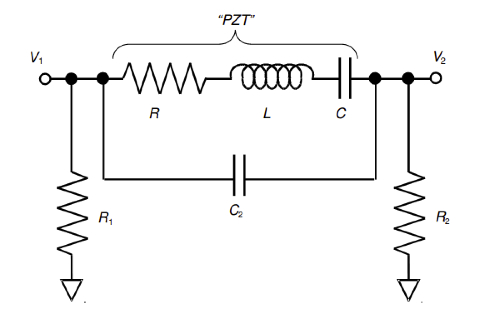
\includegraphics[width=\linewidth]{esquemapzt.jpg}
\caption{Diagrama del circuito RLC equivalente para el piezoel\'ectrico de cuarzo. Se muestra la capacidad adicional $C_{2}$ introducida por las placas de metal agregadas al cristal; $R_{1}$ y $R_{2}$ resistencias arbitrarias y los voltajes de entrada y salida $V_{1}$ y $V_{2}$, respectivamente.}
\label{fig:esquemapzt}
\end{figure}

Gracias al modelado del material de cuarzo como un circuito RLC, podemos calcular algunas de sus propiedades para poder caracterizarlo, siendo de nuestro inter\'es los par\'ametros $R$, $L$, $C$ y $C_{2}$ del mismo. Para eso, veamos algunas propiedades de los circuitos mencionados, por ejemplo su admitancia, dada por la siguiente ecuaci\'on:

\begin{equation}
\label{eq:admitancia}
Y = \frac{1}{Z} = \frac{R}{R^{2} + \Omega^{2}} + j(\omega C_{2} - \frac{\Omega}{R^{2} + \Omega^{2}})
\end{equation}

siendo $Z$ la impedancia y $\Omega = \omega L - \frac{1}{\omega C}$.

La transferencia de energ\'ia del circuito est\'a dada por: 

\begin{equation}
\label{eq:transferencia}
T = \frac{|V_{2}|}{|V_{1}|} = \frac{R_{2}}{R_{2} + Z}
\end{equation}

donde $R_{2}$ es una resistencia arbitraria en el circuito, $V_{1}$ y $V_{2}$ los voltajes de entrada y salida respectivamente.
Evaluando la transferencia en la frecuencia de resonancia $\omega_{r}$ del sistema se obtiene la siguiente ecuaci\'on, la cual nos permitir\'a calcular la resistencia $R$:

\begin{equation}
\label{eq:transferenciar}
T(\omega_{r}) = \frac{R_{2}}{R_{2} + R}
\end{equation}

\par
El par\'ametro $L$ se define a partir del c\'alculo del factor de calidad  $Q$ del cristal. Este factor est\'a dado por la ecuaci\'on:

\begin{equation}
\label{eq:merito}
Q = \frac{\omega_{r}}{\Delta \omega} = \frac{\omega_{r}L}{R_{2} + R}
\end{equation}

donde $\Delta \omega$ es el ancho de la campana de resonancia. \newline

\par
Por \'ultimo, se pueden obtener los valores para la frecuencia de resonancia $\omega_{r}$ y antirresonancia $\omega_{a}$ experimentalmente mediante las siguientes ecuaciones, teniendo en cuenta que $C_{2}$ es muy peque\~no comparado con $C$:

\begin{equation}
\label{eq:wr}
\omega_{r} = \frac{1}{\sqrt{LC}}
\end{equation}

\begin{equation}
\label{eq:wa}
\omega_{a} = \sqrt{\frac{1}{L}(\frac{1}{C} + \frac{1}{C_{2}})}
\end{equation}

%------------------------------------------------

\section{Dispositivo experimental}

Los instrumentos de laboratorio utilizados fueron:
\begin{itemize}
\item 
\label{Laser} PC con software MATLAB para la adquisici\'on y an\'alisis de los datos.
\item Generador de funciones Tektronix AFG3021B.
\item Osciloscopio Tektronix TDS1002B.
\item Amplificador Lock-In Stanford Research Systems SR830DSP, con interfaz GPIB.
\item Cables BNC.
\item Cristal piezoel\'ectrico de cuarzo.
\end{itemize}


En esta experiencia, se trabajo con un cristal piezoel\'ectrico de base cuadrada, cortado a +5 \degree respecto de uno de sus ejes; contenido en una base cerrada de acr\'ilico. En dos de las caras del cristal, se encontraban dispuestos electrodos de metal, cada uno con un alambre soldado, cada uno de los cuales estaban en serie con una resistencia de 10 K$\Omega$. En la siguiente figura se puede ver un esquema del dispositivo utilizado:

\begin{figure}[H]
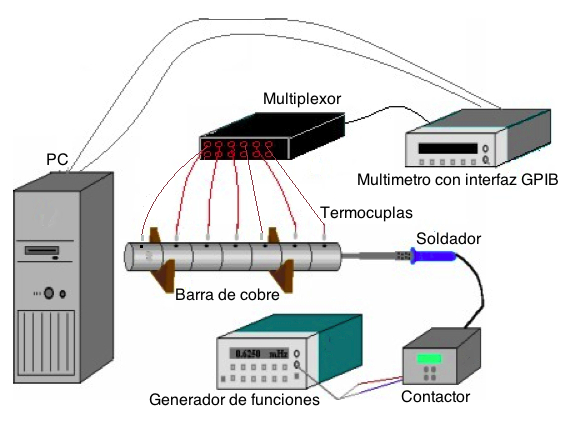
\includegraphics[width=\linewidth]{dispexp.jpg}
\caption{Esquema del dispositivo experimental utilizado. En primera instancia, en lugar del amplificador se dispuso un osciloscopio.}
\label{fig:dispexp}
\end{figure}

En uno de los alambres mencionados, se utiliz\'o el generador de funciones para aplicar una se\~nal de entrada $V_{1}$ de amplitud 2 Vpp y frecuencia variable. Luego, sobre el otro alambre se registr\'o la se\~nal de salida $V_{2}$, en primera instancia con el osciloscopio y luego con el amplificador lock-in. Con \'este \'ultimo tambi\'en se obtuvo la diferencia de fase entre la se\~nal de entrada y la de salida. Cabe aclarar que, para poder establecer una senal de referencia requerida por el amplificador lock-in, se conecto una de las salidas del generador de funciones con la entrada de referencia del amplificador.


Finalmente, se conectaron el osciloscopio (mediante cable USB) y el amplificador (mediante interfaz GPIB) a una PC con software MATLAB,    con el cual se ejecut\'o un script para poder recolectar y analizar los datos enviados por los equipos mencionados.



\begin{table}[H]
\centering
\caption{Posici\'on de cada termocupla en la barra con respecto al extremo en contacto con el soldador (posici\'on 0).}
\label{tab:posiciones}
\begin{tabular}{|c|c|}
\hline
Termocupla & Posici\'on ( $\pm 0,1 cm$) \\ \hline
1 K & 4,1\\ \hline
2 K & 8,6\\ \hline
3 J & 13,4\\ \hline
4 J & 17,1\\ \hline
5 J & 22,0\\ \hline
6 J & 29,2\\ \hline
7 J & 36,4\\ \hline
\end{tabular}
\end{table}

%------------------------------------------------
\section{Resultados y an\'alisis}

Para estimar la temperatura a la cual el sistema alcanza el r\'egimen estacionario, se aliment\'o al soldador con una onda cuadrada de per\'iodo $\tau$ = 170 seg. y amplitud de 6,432 Vpp. durante la primera medici\'on realizada en un tiempo de 1:30 hs.; observando que la misma aumenta de manera uniforme durante \'este r\'egimen hasta oscilar alrededor de un valor fijo en cada termocupla para los \'ultimos valores de tiempo en esta medici\'on ($t \approx$ 4800 a 5000 seg.), teniendo en cuenta el error de precisi\'on de las mismas ($\pm$ 1,5 \degree C). Por ejemplo, en las termocuplas 1 y 4, $T_{Ch 1} \approx$  90 \degree C y $T_{Ch 4} \approx$ 79,2 \degree C respectivamente, como puede verse en la siguiente figura.

\begin{figure}[H]
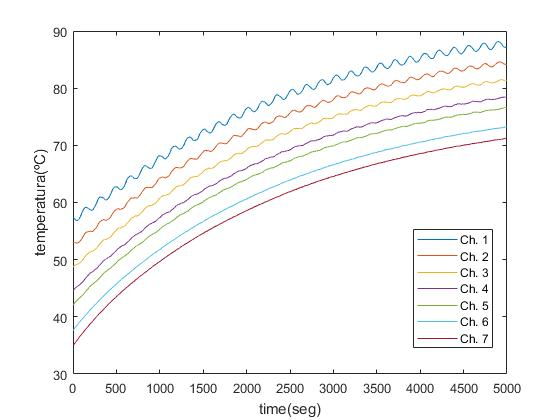
\includegraphics[width=\linewidth]{Tvst_transitorio.jpg}
\caption{Valores de temperatura en cada termocupla durante el regimen transitorio}
\label{fig:Tvst_transitorio}
\end{figure}


Luego, se deja evolucionar al sistema durante 3 horas m\'as, para poder alcanzar el r\'egimen estacionario, y se realiza la segunda medici\'on, con los mismos par\'ametros de per\'iodo y amplitud que para el transitorio.

\begin{figure}[H]
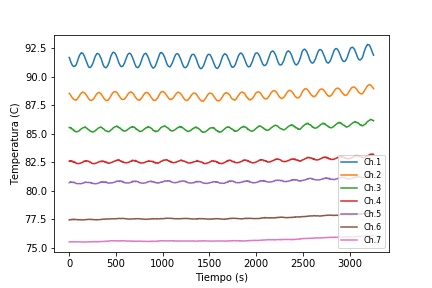
\includegraphics[width=\linewidth]{Tvst.jpg}
\caption{Valores de temperatura en funcion del tiempo para cada termocupla durante el regimen estacionario}
\label{fig:Tvst_estacionario}
\end{figure}


Podemos notar que la temperatura inicial de la termocupla 1 es de aproximadamente 91,5 \degree C, muy cercano al valor de la \'ultima medici\'on de temperatura (a $t$ = 5000 seg) para el r\'egimen transitorio. Teniendo en cuenta esto, m\'as el rango de precisi\'on mencionado en cada termocupla; nos indica que el tiempo de 3 horas utilizado para alcanzar el r\'egimen estacionario una vez comenzado el experimento fue el correcto.

\subsection{C\'alculo de la velocidad $v$ y la constante de decaimiento $\epsilon$ de la onda t\'ermica}


La velocidad de propagaci\'on de la onda de calor est\'a dada por:

\begin{equation}
\label{eq:velocidad}
v = \frac{\Delta x}{\Delta t}
\end{equation}

donde $\Delta x$ es la distancia dada por la diferencia en las posiciones de las termocuplas que figuran en la Tabla \ref{tab:posiciones}. $\Delta t$ es el tiempo que la onda de temperatura tarda en llegar de una termocupla a otra. Se trabaj\'o con los valores obtenidos con los canales 1 y 2, sin tomar en cuenta los otros canales debido a que al calcular los m\'aximos de temperatura, el algoritmo de detecci\'on de picos fallaba, mientras que la se\~nal de los canales 1 y 2 fue lo suficientemente limpia para que detecte bien los m\'aximos. A\'un as\'i, se utilizaron algunos algoritmos de optimizaci\'on, como por ejemplo, se limpi\'o el ruido de la se\~nal y cuando el programa detectaba dos m\'aximos en un lugar donde s\'olo deb\'ia haber uno, fueron promediados. \newline

\par
En la Figura \ref{fig:deltat} se puede ver un acercamiento a la diferencia temporal que hay entre el primer m\'aximo de temperatura de los canales 1 y 2. Se realiz\'o este procedimiento para todos los m\'aximos y se obtuvo una lista de diferencias temporales, la cual se promedi\'o, obteniendo: $\Delta t = (16,6 \pm 3,8)$ seg., para el error de este valor se considero la desviaci\'on est\'andar de la de la curva gaussiana centrada en el valor medio pues los errores m\'as notables se producieron en el an\'alisis de datos. La diferencia entre la posici\'on de las termocuplas 1 y 2 es: $\Delta x = (0,045 \pm 0,002)$ m., pudiendo obtener un valor para la velocidad de la onda de $v = (0,0027 \pm 0,0007) \frac{m}{seg}$, el error de este valor se obtuvo a partir de la propagaci\'on de errores.

\begin{figure}[H]
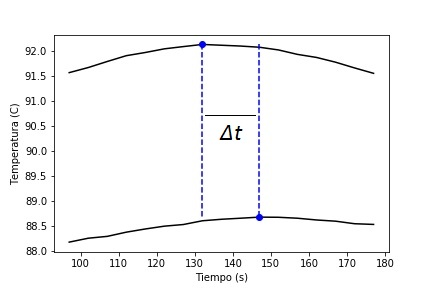
\includegraphics[width=\linewidth]{deltat.jpg}
\caption{Detalle de la diferencia de fases entre los valores m\'aximos de la temperatura en los canales 1 y 2.}
\label{fig:deltat}
\end{figure}


Para obtener el valor del coeficiente de decaimiento $\epsilon$ se calcul\'o el valor medio de la temperatura de cada termocupla, y se realizo un ajuste exponencial de la variaci\'on de temperatura en funci\'on de la posici\'on de cada una de ellas, donde se encontro que $\epsilon = (6,1 \pm 0,3) \frac{1}{m} $ (Figura \ref{fig:decaimiento}).

\begin{figure}[H]
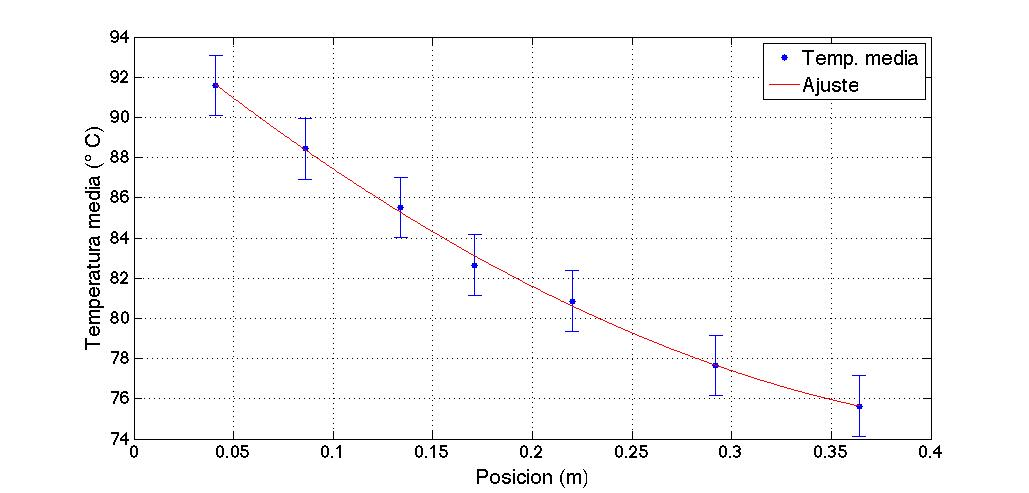
\includegraphics[width=\linewidth]{decaimiento.jpg}
\caption{Ajuste por una curva exponencial de la temperatura media en funcion de la posici\'on de cada termocupla.}
\label{fig:decaimiento}
\end{figure}

Por ultimo, mediante las ecuaciones (\ref{eq:ke}) y (\ref{eq:kv}) se encontr\'o que $\kappa_{\epsilon} = (4,9 \pm 0,7) * 10^{-4} \frac{m^{2}}{seg}$ y $\kappa_{v} = (1,2 \pm 0,7) * 10^{-4} \frac{m^{2}}{seg}$, lo que permite realizar un promedio entre ambos valores y obtener un valor aproximado de la constante de difusividad t\'ermica de $\bar{\kappa} = (3,11 \pm 0,7) * 10^{-4}  \frac{m^{2}}{seg}$.

Al utilizar la ecuaci\'on (\ref{eq:kappa}), con los datos obtenidos para la velocidad $v$ y la constante de decaimiento $\epsilon$, se obtuvo que $\kappa = (2,4 \pm 0,7) * 10^{-4} \frac{m^{2}}{seg}$, notando que existe una leve diferencia de $0.7\frac{m^{2}}{seg}$, entre el valor obtenido con $\bar{\kappa}$ con respecto al calculado mediante la ecuaci\'on mencionada.

%------------------------------------------------

\section{Conclusiones}

Para poder obtener las constantes de difusividad t\'ermica y de decaimiento de una barra de Cobre se estudi\'o la conducci\'on de calor en la misma, calentando un soldador fijado a un extremo de la misma mediante un contactor controlado por un generador de ondas emitiendo una onda cuadrada de per\'iodo $\tau$ = 170 seg. durante los r\'egimenes transitorio y estacionario. \newline

\par
Las medidas de temperatura se obtuvieron mediante termocuplas insertadas a lo largo de la barra en diferentes posiciones, con respecto a una posici\'on 0, que se eligi\'o en el extremo donde se coloc\'o el soldador. Los datos recolectados mediante el mult\'imetro conectado a dichas termocuplas permitieron calcular la velocidad $v$ de propagaci\'on de la onda y su constante de decaimiento $\epsilon$. \newline

\par
La velocidad de propagaci\'on de la onda de calor se calculo mediante la distancia $\Delta x$ entre termocuplas y $\Delta t$ es el tiempo que la onda de temperatura tarda en llegar de una termocupla a otra; obteniendo un valor de $v = (0,0027 \pm 0,0007) \frac{m}{seg}$. \newline

\par
Para la obtenci\'on del valor del coeficiente de decaimiento $\epsilon$ se calcul\'o el valor medio de la temperatura de cada termocupla, y se realizo un ajuste exponencial de la variaci\'on de temperatura en funci\'on de la posici\'on de cada una de ellas, dando $\epsilon = (6,1 \pm 0,3) \frac{1}{m}$. \newline

\par
A partir de lo mencionado en los dos p\'arrafos anteriores, fue posible determinar los factores $\kappa_{\epsilon} = (4,9 \pm 0,7) * 10^{-4} \frac{m^{2}}{seg}$ y $\kappa_{v} = (1,2 \pm 0,7) * 10^{-4} \frac{m^{2}}{seg}$, lo que permiti\'o realizar un promedio entre ambos para obtener un valor aproximado de la constante de difusividad t\'ermica de $\bar{\kappa} = (3,11 \pm 0,7) * 10^{-4}  \frac{m^{2}}{seg}$.

Podemos comparar este valor de $\bar{\kappa}$ con el calculado mediante la ecuaci\'on (\ref{eq:kappa}), siempre utilizando los datos recolectados para $v$ y $\epsilon$, con los cuales se obtuvo que $\kappa = (2,4 \pm 0,7) * 10^{-4} \frac{m^{2}}{seg}$. Se puede ver que existe una diferencia de $0.7\frac{m^{2}}{seg}$ entre el valor calculado con $\bar{\kappa}$ y $\kappa$, lo que permite que en ciertas condiciones puedan considerarse iguales. \newline

\par
Con los resultados obtenidos experimentalmente para $\kappa$, se obtuvo una diferencia del 45 \% con respecto al valor te\'orico tabulado para el Cobre, $\kappa = 1,12 * 10^{-4} \frac{m^{2}}{seg}$., que si bien se encuentra dentro del orden de magnitud propuesto por la bibliograf\'ia, creemos que se produjeron errores debido a la baja sensibilidad de las termocuplas y al c\'alculo del $\Delta t$, produciendo que la detecci\'on de m\'aximos de intensidad no sean tan exactos, afectando el c\'alculo final de los coeficientes, sobre todo de $\kappa_{\epsilon}$.


%----------------------------------------------------------------------------------------
%	REFERENCE LIST
%----------------------------------------------------------------------------------------
\newpage
\begin{thebibliography}{99} % Bibliography - this is intentionally simple in this template


\bibitem{eq:calor} A. Bodas, V. G\'andia and E. L\'opez-Baeza, \textit{An undergraduate experiment on the propagation of thermal waves}, American Journal of Physics, \textbf{66}, 528 (1998).

\bibitem{teo:kappa} W. Czarnetzki, M. Wandelt, and W. Roetzel, \textit{Thermal wave analysis for measurements of thermal diffusivity, Proceedings of the Joint Conference 1996: IEEE Instrumentation and Measurement Technology Conference and IMEKO Technical Committee 7}, Brussels, Belgium, 4-6 June 1996 (IEEE, New York, 1996), p\'ag. 1195.
 
\end{thebibliography}


%----------------------------------------------------------------------------------------

\end{document}